
%<<setup-child, include = FALSE>>=
%library(knitr)
%library(microbenchmark)
%library(reshape2)
%library(ggplot2)
%set_parent("../style/preamble.Rnw")
%
%set.seed(1)
%@
\input{../../2021/style/preamble4tex}
% dependencies: amsmath, amssymb, dsfont
% math spaces
\ifdefined\N
\renewcommand{\N}{\mathds{N}} % N, naturals
\else \newcommand{\N}{\mathds{N}} \fi
\newcommand{\Z}{\mathds{Z}} % Z, integers
\newcommand{\Q}{\mathds{Q}} % Q, rationals
\newcommand{\R}{\mathds{R}} % R, reals
\ifdefined\C
\renewcommand{\C}{\mathds{C}} % C, complex
\else \newcommand{\C}{\mathds{C}} \fi
\newcommand{\continuous}{\mathcal{C}} % C, space of continuous functions
\newcommand{\M}{\mathcal{M}} % machine numbers
\newcommand{\epsm}{\epsilon_m} % maximum error

% counting / finite sets
\newcommand{\setzo}{\{0, 1\}} % set 0, 1
\newcommand{\setmp}{\{-1, +1\}} % set -1, 1
\newcommand{\unitint}{[0, 1]} % unit interval

% basic math stuff
\newcommand{\xt}{\tilde x} % x tilde
\newcommand{\argmin}{\mathop{\mathrm{arg\,min}}} % argmin
\newcommand{\argmax}{\mathop{\mathrm{arg\,max}}} % argmax
\newcommand{\argminlim}{\argmin\limits} % argmin with limits
\newcommand{\argmaxlim}{\argmax\limits} % argmax with limits
\newcommand{\sign}{\operatorname{sign}} % sign, signum
\newcommand{\I}{\mathbb{I}} % I, indicator
\newcommand{\order}{\mathcal{O}} % O, order
\newcommand{\bigO}{\mathcal{O}} % Big-O Landau
\newcommand{\littleo}{{o}} % Little-o Landau
\newcommand{\pd}[2]{\frac{\partial{#1}}{\partial #2}} % partial derivative
\newcommand{\floorlr}[1]{\left\lfloor #1 \right\rfloor} % floor
\newcommand{\ceillr}[1]{\left\lceil #1 \right\rceil} % ceiling
\newcommand{\indep}{\perp \!\!\! \perp} % independence symbol

% sums and products
\newcommand{\sumin}{\sum\limits_{i=1}^n} % summation from i=1 to n
\newcommand{\sumim}{\sum\limits_{i=1}^m} % summation from i=1 to m
\newcommand{\sumjn}{\sum\limits_{j=1}^n} % summation from j=1 to p
\newcommand{\sumjp}{\sum\limits_{j=1}^p} % summation from j=1 to p
\newcommand{\sumik}{\sum\limits_{i=1}^k} % summation from i=1 to k
\newcommand{\sumkg}{\sum\limits_{k=1}^g} % summation from k=1 to g
\newcommand{\sumjg}{\sum\limits_{j=1}^g} % summation from j=1 to g
\newcommand{\summM}{\sum\limits_{m=1}^M} % summation from m=1 to M
\newcommand{\meanin}{\frac{1}{n} \sum\limits_{i=1}^n} % mean from i=1 to n
\newcommand{\meanim}{\frac{1}{m} \sum\limits_{i=1}^m} % mean from i=1 to n
\newcommand{\meankg}{\frac{1}{g} \sum\limits_{k=1}^g} % mean from k=1 to g
\newcommand{\meanmM}{\frac{1}{M} \sum\limits_{m=1}^M} % mean from m=1 to M
\newcommand{\prodin}{\prod\limits_{i=1}^n} % product from i=1 to n
\newcommand{\prodkg}{\prod\limits_{k=1}^g} % product from k=1 to g
\newcommand{\prodjp}{\prod\limits_{j=1}^p} % product from j=1 to p

% linear algebra
\newcommand{\one}{\bm{1}} % 1, unitvector
\newcommand{\zero}{\mathbf{0}} % 0-vector
\newcommand{\id}{\bm{I}} % I, identity
\newcommand{\diag}{\operatorname{diag}} % diag, diagonal
\newcommand{\trace}{\operatorname{tr}} % tr, trace
\newcommand{\spn}{\operatorname{span}} % span
\newcommand{\scp}[2]{\left\langle #1, #2 \right\rangle} % <.,.>, scalarproduct
\newcommand{\mat}[1]{\begin{pmatrix} #1 \end{pmatrix}} % short pmatrix command
\newcommand{\Amat}{\mathbf{A}} % matrix A
\newcommand{\Deltab}{\mathbf{\Delta}} % error term for vectors

% basic probability + stats
\renewcommand{\P}{\mathds{P}} % P, probability
\newcommand{\E}{\mathds{E}} % E, expectation
\newcommand{\var}{\mathsf{Var}} % Var, variance
\newcommand{\cov}{\mathsf{Cov}} % Cov, covariance
\newcommand{\corr}{\mathsf{Corr}} % Corr, correlation
\newcommand{\normal}{\mathcal{N}} % N of the normal distribution
\newcommand{\iid}{\overset{i.i.d}{\sim}} % dist with i.i.d superscript
\newcommand{\distas}[1]{\overset{#1}{\sim}} % ... is distributed as ...


\begin{document}

\lecturechapter{4}{Introduction to Big O}
\lecture{CIM1 Statistical Computing}

\begin{vbframe}{Efficiency of algorithms}

We are interested in the \textbf{efficiency} of algorithms. Efficiency can be associated with different attributes such as
  \begin{itemize}
    \item CPU runtime
    \item Memory usage
    \item Memory usage on the hard drive
  \end{itemize}

\lz

We will mainly focus on the \textbf{runtime behavior} of algorithms.

\end{vbframe}

\begin{vbframe}{The Big O Notation}

\begin{itemize}
\item When we are interested in the complexity of an algorithm, we are \textbf{not} interested in the exact number of operations, but rather in the relationship of the number of operations to the size of the problem.
  \item Usually one is interested in the \textbf{worst case}:\\
  what is the maximum number of operations for a given problem size?
  \item The Big O notation (also called Bachmann-Landau notation) is used in mathematics
  and computer science to classify algorithms according to how their run time or space requirements grow as the input size grows.
\end{itemize}

% \begin{footnotesize}
% \textbf{Achtung:} Es ist üblich, obere Schranken for die Laufzeit (also den Worst Case) über alle Probleminstanzen zu betrachten. Da in der Praxis meist nur eine bestimmte Probleminstanz betrachtet wird, kann die tatsächliche Laufzeit deutlich kürzer sein als im Worst Case Szenario.
% \end{footnotesize}

\end{vbframe}

\begin{vbframe}{input sizes}

An analysis of complexity depends on how you specify the input size of a problem.

\lz

Typical input sizes are:

\begin{itemize}
\item Number of elements of a list
\item Number of bits of a number
\item Number of nodes in a graph
\item Number of rows / columns of a matrix
\end{itemize}

\end{vbframe}


\begin{vbframe}{Introductory example}
\lz
\footnotesize
\begin{verbbox}
isElement = function(xs, el) {
  for (x in xs) {
    if (identical(x, el))
      return(TRUE)
  }
  return(FALSE)
}
\end{verbbox}
\col
\lz
\begin{verbbox}
## expr mean
## 1 isElement(1:1000, 1000L) 308.286
## 2 isElement(1:2000, 2000L) 626.519
## 3 isElement(1:5000, 5000L) 1684.067
## 4 isElement(1:10000, 10000L) 3137.450
\end{verbbox}
\col
%<<>>=
%isElement = function(xs, el) {
%  for (x in xs) {
%    if (identical(x, el))
%      return(TRUE)
%  }
%  return(FALSE)
%}
%@
%
%<<echo=FALSE>>=
%summary(microbenchmark(
%  isElement(1:1000, 1000L),
%  isElement(1:2000, 2000L),
%  isElement(1:5000, 5000L),
%  isElement(1:10000, 10000L)))[, c("expr", "mean")]
%@

\normalsize
\framebreak

\begin{itemize}
  \item The input size of the problem is $n$ being the length of vector $xs$.
  \item The order of the function is $\order(n)$ (worst case).
  \item That is: \\
  If we were to evaluate the function for different $xs$ and visualize the runtime in
  a graph, it would show that the runtime depends linearly on the number of elements in $xs$.
   \item For example, if we always consider the vector \code{xs = 1:n} and test for the number \code{1}, our function would obviously be much faster than $\order(n)$.
\end{itemize}


\framebreak

\begin{center}
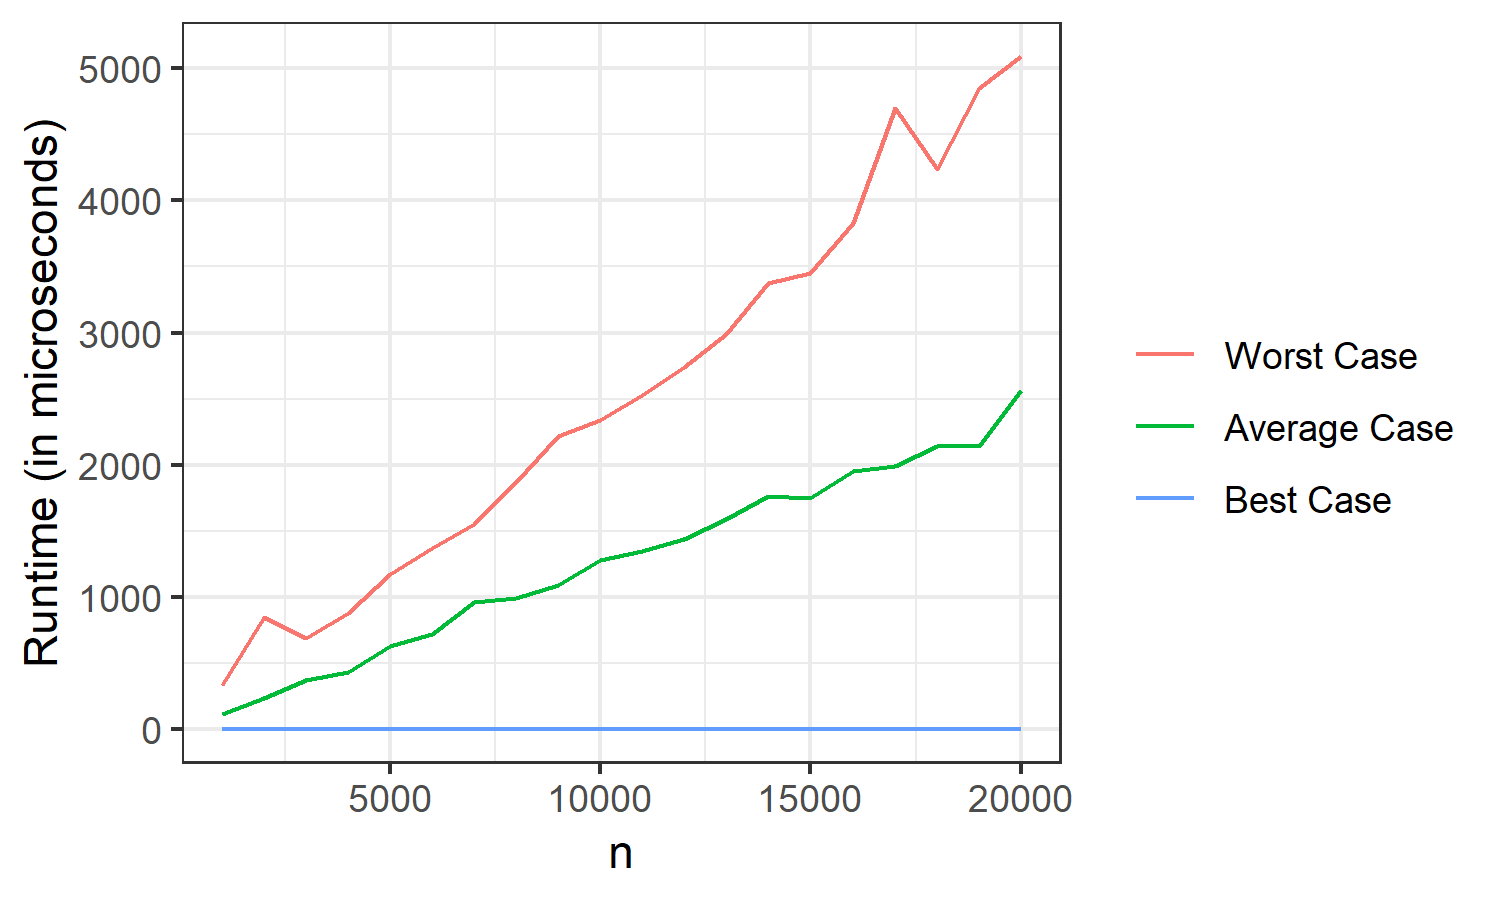
\includegraphics[width=0.8\textwidth]{figure_man/runtime.png}
\end{center}

\begin{footnotesize}
In the best case, we always access the first element of the list. The runtime is constant. In the worst case we access the $n$-th element of the list - so $n$ elements have to be evaluated. On average $\frac{n}{2}$ evaluations are needed.
\end{footnotesize}


\framebreak

\begin{itemize}
  \item In general, the Big-O notation is used to describe the \textbf{worst case} and
  thus represents an upper bound.
  \item Another common performance measure is the \textbf{average case} runtime.
  \item Many algorithms have poor worst-case performance, but good average-case performance and are therefore quite practicable depending on the application.
  \item Less common is the best case performance, i.e. the behavior of the algorithm under optimal conditions.
\end{itemize}


\end{vbframe}

\begin{vbframe}{Formal definition}

Let $f, g: \R \to \R$ be two functions.

\lz

We define
$$
f(x) \in \order(g(x)) \quad \text{for } x \to \infty
$$
if and only if 2 positive real numbers $M$ and $x_0$ exist, such that
$$
|f(x)| \leq M \cdot |g(x)| \quad \text{for all } x > x_0.
$$

\lz

Intuition: $f$ does not grow faster than $g$.

\lz

\textbf{Comment:} Often the above definition is abbreviated by $f \in \order(g)$.

\framebreak

\textbf{Example:} We consider the function $f(x) = 3 x^3 + x^2 + 100 \sin(x)$.

\lz
\begin{center}
\begin{figure}
  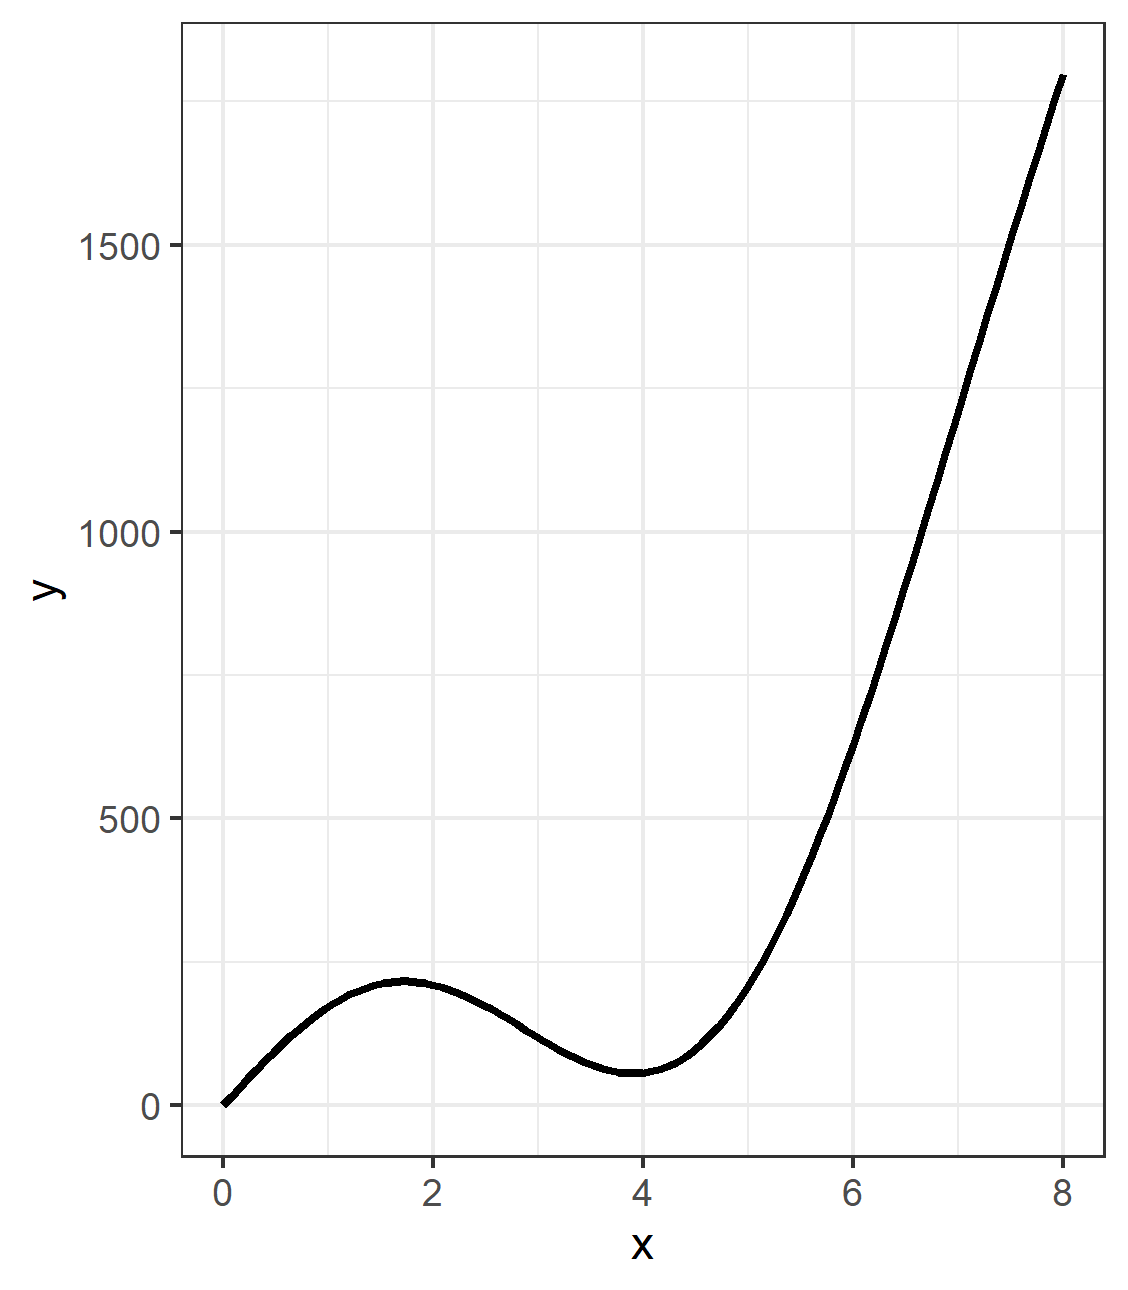
\includegraphics[height = 6cm, width = 6cm]{figure_man/Example1.png}
\end{figure}
\end{center}

\end{vbframe}

\begin{vbframe}{Formal definition}

For large $x$, $f(x)$ is well above $1 \cdot g(x) = 1 \cdot x^3$

\lz

\begin{center}
\begin{figure}
  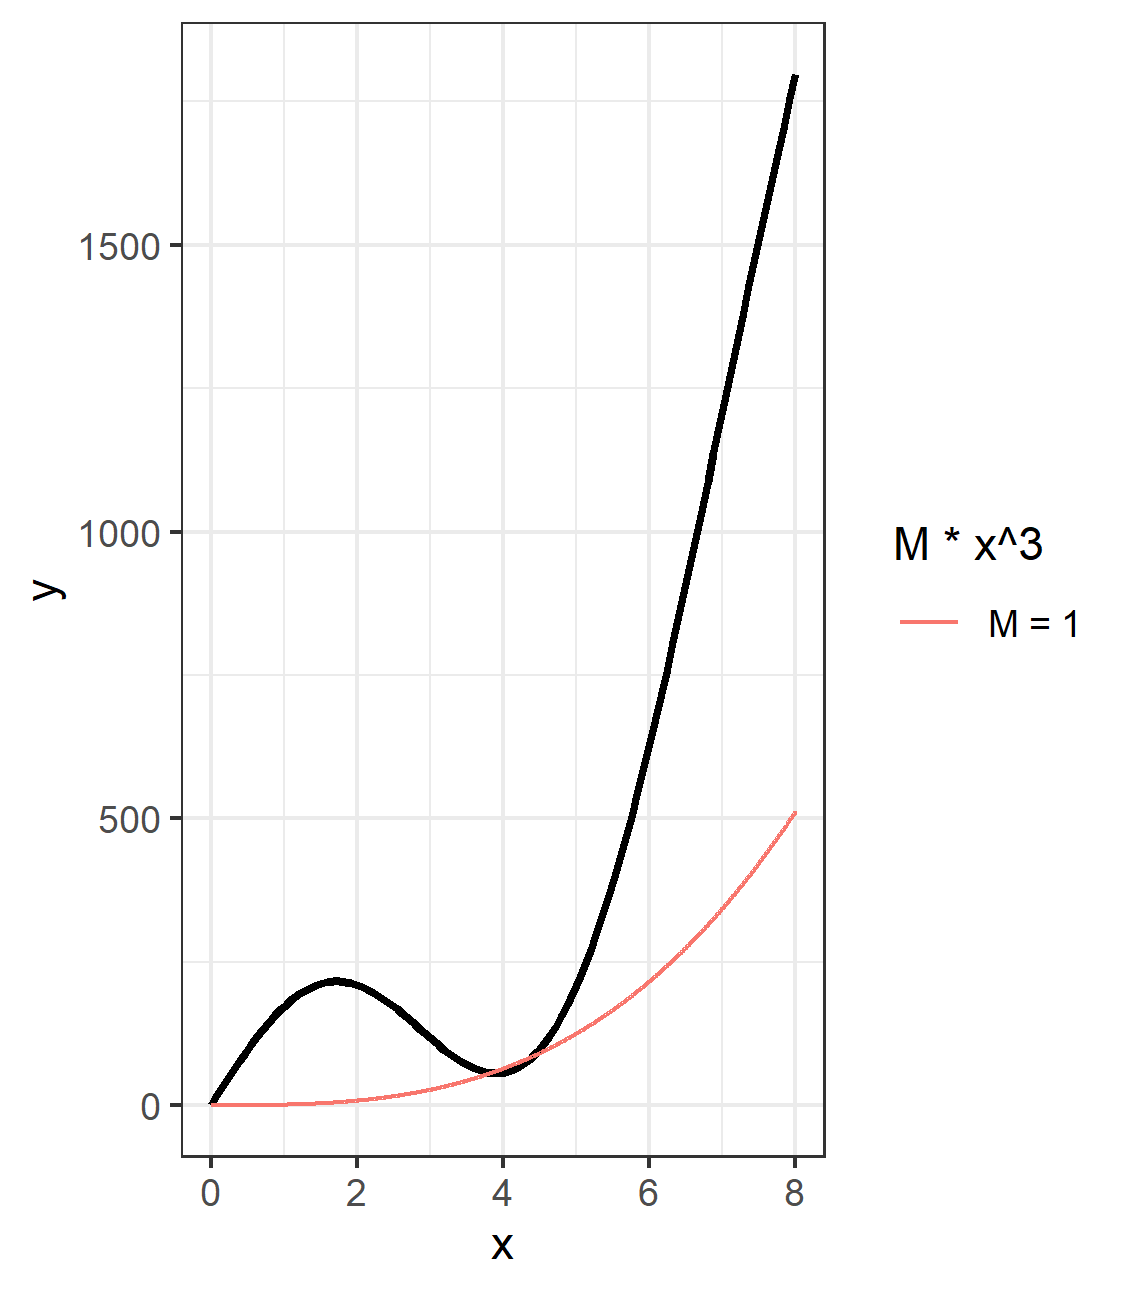
\includegraphics[height = 6cm, width = 8cm]{figure_man/Example1b.png}
\end{figure}
\end{center}


\framebreak

We are now looking at the relationship between $f(x)$ and $M\cdot x^3$ for $M = 1, 2, 3, ...$. In the graph below we can see that $f(x)$ runs entirely \textbf{beneath} $4 \cdot x^3$ for $x$ values greater than $\approx 3$,. This means $f$ grows cubic: $f \in \order(x^3)$.


\begin{center}
\begin{figure}
  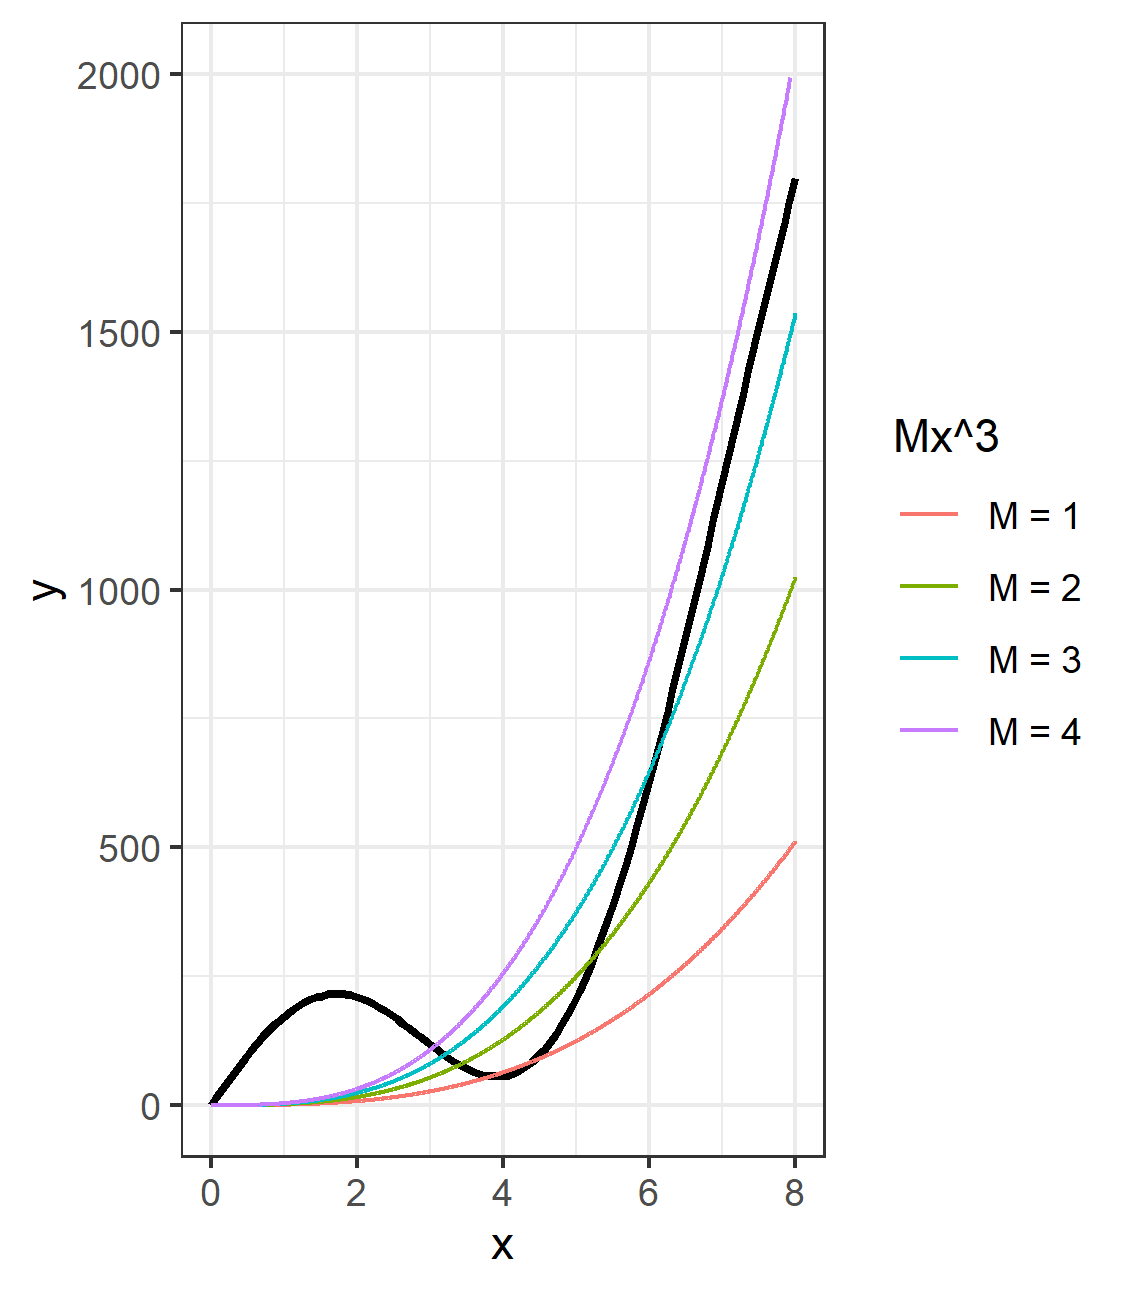
\includegraphics[height = 5.5cm, width = 8cm]{figure_man/Example1c.png}
\end{figure}
\end{center}

\framebreak

Mathematical derivation:
\begin{eqnarray*}
|f(x)| &=& | 3 x^3 + x^2 + 100 \sin(x) | \le 3 \cdot |x|^3 + x^2 + 100 \underbrace{|\sin(x)|}_{\le 1} \\ &\le& 3 \cdot |x|^3 + \underbrace{x^2}_{\le |x|^3 \text{ for } x > 1} + 100 \\ %\qquad
&\le& 4 |x|^3 + 100 \text{  for  } x > 1.
\end{eqnarray*}

Since $100 \le 4 |x|^3$ for $x > \sqrt[3]{25} \approx 2.9$ it follows

$$
|f(x)| \le 4 |x^3| \text{  for  } x > x_0 := \sqrt[3]{25},
$$

or in short $f \in \order(x^3)$, which corresponds to our graphical derivation.


\framebreak

For functions $f, g: X \to \R$, $X\subset \R$ you can also use this notation to examine the behavior of the function $f$ at a certain point $a \in X$ (often $a=0$):

\begin{eqnarray*}
  f(x) &\in& \order(g(x)) \quad \text{for } x \to a \in \R \\
  % &\iff& \\
  % |f(x)| &\leq& M \cdot |g(x)| \\
\end{eqnarray*}
if 2 positive real numbers $M$ and $d$ exist, such that

$$
|f(x)| \leq M \cdot |g(x)| \quad \text{for } |x-a| < d.
$$

\framebreak

  If $g(x)$ is not equal to 0 and is close enough to $a$ for values of $x$, then both definitions can be expressed using the limes superior:

\begin{eqnarray*}
  f(x) &\in& \order(g(x)) \quad \text{for } x \to a \in \R \\
  &\iff& \\
  \lim_{x \rightarrow a} \sup \frac{|f(x)|}{|g(x)|} &<& \infty\\
\end{eqnarray*}

\end{vbframe}

\begin{vbframe}{Notation}

  \begin{itemize}
    \item When we talk about the order of a function, we write
    $$f \in \order(n^2)$$
    \item A second, more commonly used notation is
        $$f = \order(n^2)$$
        although it is formally incorrect:\\
    $n^2 = \order(n^2)$ and $n^2/2 = \order(n^2)$, but $n^2 \neq n^2/2$
    \item In this context, the \enquote{$=$} is not intended to be a sign of equality, but a simple \enquote{is}
  \end{itemize}
\end{vbframe}

\begin{vbframe}{classes of functions}

\begin{center}
  \begin{tabular}{ c | c}
  Notation & Description \\
  \hline
  $\order(1)$ & constant \\
  $\order(\log(n))$ & logarithmic \\
  $\order((\log(n))^c)$ & polylogarithmic \\
  $\order(n)$ & linear \\
  $\order(n^2)$ & square \\
  $\order(n^c)$ & polynomial \\
  $\order(c^n)$ & exponential
  \end{tabular}
\end{center}

The table is sorted from slow to fast growing for $c > 1$

\framebreak

\lz

\begin{center}
\begin{figure}
  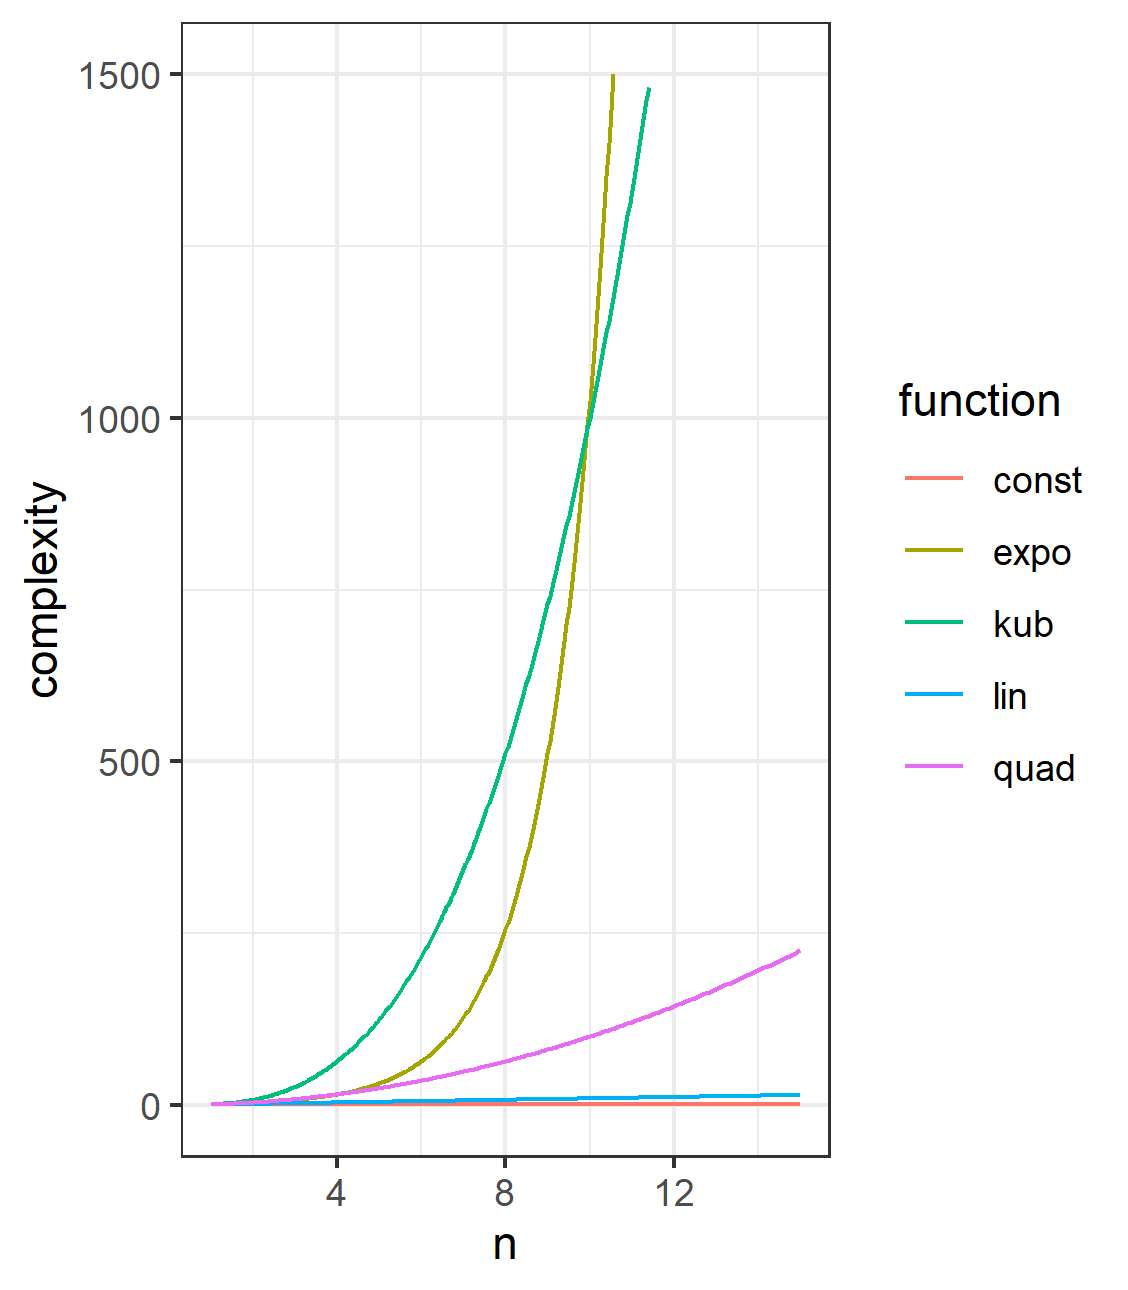
\includegraphics[height = 8cm, width = 9cm]{figure_man/classes.png}
\end{figure}
\end{center}

\end{vbframe}



\endlecture
\end{document}
